\section{mbeddr Debugger}

mbeddr comes with a debugger, which allows user to debug code written
with mbeddr. Since mbeddr is extensible, the debugger is extensible as well for
enabling debugging of new language extensions.

mbeddr programs can be composed of different languages and form this way
mixed-languages programs. The debugger for those languages is composed at
debug-time and allows users to debug their code at the extension-level,
where the language extensions are used. The debug support is enabled by lifting
the call stack and program state from the base level to the extension level
(see \fig{infoFlow}). In contrast, stepping and breakpoints are translated vice
versa.

\begin{figure}[h]
  \vspace{-2mm}
  \centering
    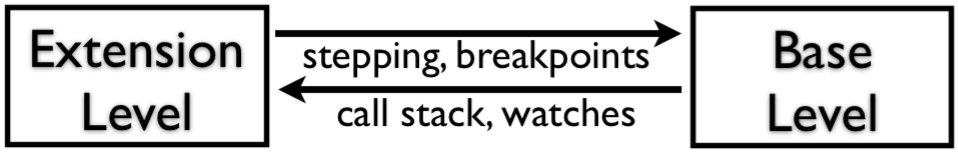
\includegraphics[width=7cm]{./figures/two-levels.png} 
    \vspace{-2mm}
    \caption{Flow of debug information between base and
    extension level~\cite{DBLP:conf/adaEurope/AdaEuropeDeb}}
  \label{infoFlow}
  \vspace{-2mm}
\end{figure}


\subsection{Architecture}

The debugger architecture can be separated into two different aspects: First, a
\ac{DSL} and a set of interfaces for describing the debugging semantics of
language constructs. Second, a runtime for executing those descriptions and this
way performing the mapping described in the~\fig{infoFlow}. 

You can find further information about the architecture and how it is
implemented with \ac{MPS} in \cite{DBLP:conf/adaEurope/AdaEuropeDeb}. In this
section we discuss the specification part, since that is essential for
understanding how debuggers are build and later tested.

\fig{specabs} shows the meta-model used for specifying debugging semantics of
language constructs. Each node is represented in \ac{MPS} by an interface, which
is implemented by the respective language construct.

\noindent \textbf{Breakpoints} \ic{Breakable}s are consturcts on which we can
set breakpoints, \eg statements.

\noindent \textbf{Watchables} \ic{WatchProvider} is something that is either
translated to a lower level watchable (\eg a global variable) or represents a watchable on the
extension-level.
Those \ic{WatchProvider}s live inside \ic{WatchProviderScope} (\eg a
statement list), which can be nested. 

\noindent \textbf{Stepping} \ic{Steppable} is something we can step
over or into (\eg an expression statement). A so called \ic{SteppingStrategy} is
a reusable implementation of a specific stepping behavior. It describes based on
setting breakpoints (the approach is based on~\cite{Wu06grammar}) where
execution should suspend after performing a specific stepping command.
\ic{Steppable}s can contain \ic{StepIntoable}s
to which the step into command is delegated (\eg a function call).
\ic{Steppable} can be contained inside a \ic{SteppableComposite} (\eg a
statement list).

\noindent \textbf{Call Stack} A \ic{StackFrameContributor} is
something that has callable semantics on the extension-level or is
translated to a lower-level callable. While the latter category does not
contribute any \ic{StackFrame}s to the call stack, the other category
contributes one to many \ic{StackFrame}s.






\begin{figure}[h]
  \vspace{-2mm}
  \centering
    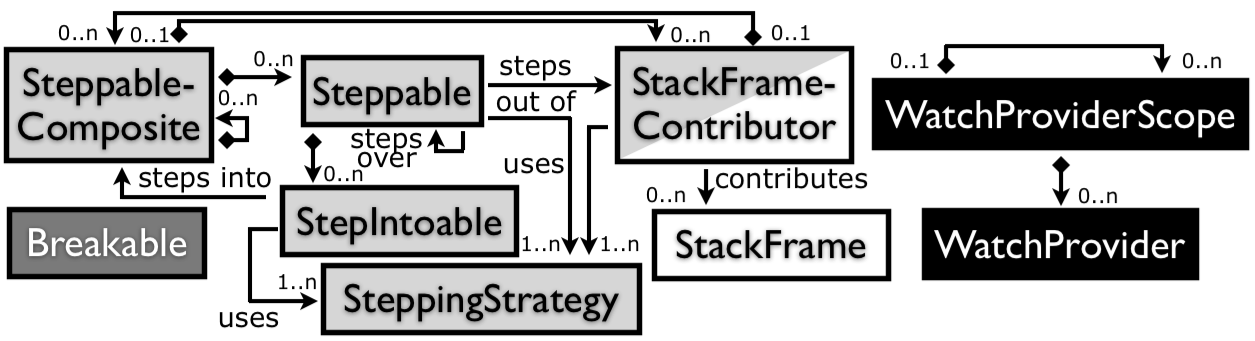
\includegraphics[width=9cm]{./figures/debugger-concepts.png} 
    \vspace{-2mm}
    \caption{Meta-model used for specying the debugging semantics of language
    constructs~\cite{DBLP:conf/adaEurope/AdaEuropeDeb}. Colors indicate the
    different aspects.} 
  \label{specabs}
  \vspace{-2mm}
\end{figure}

The specification \ac{DSL} is a language extension for MPS' Base Language,
which is an implementation of Java. It is used for describing three
debugging aspects: stepping, lifting of call stack and program state. Further
information about the language can be found in
\cite{DBLP:conf/adaEurope/AdaEuropeDeb}. We will later use this \ac{DSL} for
building debugging support for our two language extensions. 


\subsection{Building Debugging Behavior}

We describe in this section the implementation of debugging behavior for the
lanuages described in \sect{languageImplementation}. The mbeddr debugger
comes with a \ac{DSL} for specifying the debugging behavior. 
We will use the language in this section for
building debug support for both languages from \sect{languageImplementation}.

\parhead{Breakpoints} We want to be able to set breakpoints on instances of
\ic{ForEachStatement}, \ic{AssertStatement}, \ic{ItExpression}and
\ic{ExecuteTestExpression}.
For doing so, we need to implement the marker interface \ic{IBreakable}. 
Since the first two concepts
are derived from \ic{Statement} and this concept already implements this
interface, we can already set breakpoints on instances of them. The latter two
concepts will always live inside a statement derived
from \ic{Statement}. Hence, no further work is necessary.

\parhead{Call Stack} For lifting the call stack we need to specify, which
concepts have callable semantics or are generated to C functions. First applies
to \ic{TestCase}, which has callable semantics, but is also trasnalted to a C
function. In contrast, \ic{ExecuteTestExpression} does not have callable
semantics, but is translated to a C function. Other concepts are not
related to the call stack.

\ic{TestCase} , \ic{ExecuteTestExpression} \ic{IStackFrameContributor}






\parhead{Stepping}
\ic{AsserStatement}
\ic{}
\ic{ExecuteTestExpression}

\parhead{Watches}

\ic{TestCase}
\ic{ExecuteTestExpression}

